\documentclass[11pt]{article}

\usepackage{amssymb,amsmath,amsfonts,amsthm}
\usepackage{latexsym}
\usepackage{graphics}
\usepackage{indentfirst}
\usepackage{lmodern}
\usepackage{hyperref}
\usepackage{mathrsfs}
\usepackage{array}
\usepackage{mathtools}
\usepackage{graphicx}
\usepackage{setspace}
\usepackage{enumerate}
\usepackage{tikz}
\usepackage{url,color}
\usepackage{chngcntr}
\usepackage{multicol}
\usepackage{comment}
\usepackage{float} 
\usepackage{algpseudocode}
\usepackage{subcaption}
\usepackage[ruled]{algorithm2e}

\AtBeginEnvironment{algorithm}{\setstretch{1.2}}

\setlength{\textwidth}{15.5cm} \setlength{\headheight}{0.5cm} \setlength{\textheight}{21.5cm}
\setlength{\oddsidemargin}{0.25cm} \setlength{\evensidemargin}{0.25cm} \setlength{\topskip}{0.5cm}
\setlength{\footskip}{1.5cm} \setlength{\headsep}{0cm} \setlength{\topmargin}{0.5cm}


\newtheorem{innercustomthm}{Theorem}
\newenvironment{customthm}[1]
  {\renewcommand\theinnercustomthm{#1}\innercustomthm}
  {\endinnercustomthm}
\newtheorem{innercustomlem}{Lemma}
\newenvironment{customlem}[1]
  {\renewcommand\theinnercustomlem{#1}\innercustomlem}
  {\endinnercustomlem}
\newtheorem{innercustomcor}{Corollary}
\newenvironment{customcor}[1]
  {\renewcommand\theinnercustomcor{#1}\innercustomcor}
  {\endinnercustomcor}
\newtheorem{innercustompro}{Proposition}
\newenvironment{custompro}[1]
  {\renewcommand\theinnercustompro{#1}\innercustompro}
  {\endinnercustompro}
\newtheorem{innercustomconj}{Conjecture}
\newenvironment{customconj}[1]
  {\renewcommand\theinnercustomconj{#1}\innercustomconj}
  {\endinnercustomconj}

  
\newtheorem{theorem}{Theorem}[section]
\newtheorem{lemma}{Lemma}[section]
\newtheorem{proposition}{Proposition}[section]
\newtheorem{corollary}{Corollary}[section]
\newtheorem{claim}{Claim}[section]
\newtheorem{conjecture}{Conjecture}[section]
\newtheorem{hypothesis}{Hypothesis}[section]
\newtheorem{assumption}{Assumption}[section]
\newtheorem{remark}{Remark}[section]
\newtheorem{example}{Example}[section]
\newtheorem{problem}{Problem}[section]
\newtheorem{definition}{Definition}[section]
\newtheorem{question}{Question}[section]
\newtheorem{answer}{Answer}[section]
\newtheorem{condition}{Condition}[section]

\newcommand{\N}{\mathbb{N}}
\newcommand{\Z}{\mathbb{Z}}
\newcommand{\E}{\mathbb{E}}
\newcommand{\Q}{\mathbb{Q}}
\newcommand{\R}{\mathbb{R}}
\newcommand{\C}{\mathbb{C}}
\newcommand{\Var}{\mathrm{Var}}
\newcommand{\Cov}{\mathrm{Cov}}
\newcommand{\Lip}{\mathrm{Lip}}
\newcommand{\ran}{\mathrm{ran}}
\newcommand{\dc}{\chi_{_D}}
\newcommand{\bl}{\Box_{i=1}^{d}}
\newcommand{\khat}{\widehat{k}}
\newcommand{\col}{\mathrm{col}}
\newcommand{\norm}[1]{\left\lVert#1\right\rVert}



\newcommand{\F}[1]{\mathcal{F}_{#1}} 
\newcommand{\B}{\mathcal{B}} %Markov basis
\newcommand{\fiber}[1]{\mathcal{F}_{#1}} %Fiber
\newcommand{\Mbasis}{\mathcal{B}} %Markov basis
\newcommand{\Lbasis}{\mathcal{L}} %Lattice basis
\newcommand{\polytope}{P} % Polytope



%---------------- MDP - RL notation ----------------
\newcommand{\St}{\mathcal{S}} %State Space
\newcommand{\At}{\mathcal{A}} %Action Space
\newcommand{\Dt}{\mathcal{D}} %Admissable state-action pairs
\newcommand{\Qt}{p} % transition kernel
\newcommand{\Ss}{\mathcal{S}_\sigma}  %Action space sigma algebra
\newcommand{\As}{\mathcal{A}_\sigma} %State space sigma algebra
\newcommand{\Tt}{\mathcal{T}} %Time horizon
\newcommand{\EXP}{\mathbb{E}}
\newcommand{\filtration}[1]{\mathcal{I}_{#1}}


\allowdisplaybreaks


\begin{document}


%%%%%%%%%%%%%%%%%%%%%%%%%    Title and Authors
\title{Notes: A Diffusion Model for Political Redistricting}

\author{Alaittin K\i rt\i \c{s}o\u{g}lu}

\footnotetext[1]{Department of Applied Mathematics, Illinois Institute of Technology, Chicago, IL 60616. E-mail: {\tt {kirtisoglu@hawk.iit.edu}}}

\maketitle

%%%%%%%%%%%%%%%%%%%%%%%%%    Contents
\tableofcontents

\newpage

%%%%%%%%%%%%%%%%%%%%%%%%%    Abstract
%\begin{abstract}
%\end{abstract}

%%%%%%%%%%%%%%%%%%%%%%%%%

\section{Introduction}

Political redistricting seeks a partition of a geographic region into electoral districts satisfying legal, demographic, and geometric requirements such as contiguity, population balance, compactness, and
preservation of communities of interest.  Computational approaches typically model the problem on a dual adjacency graph $G=(V,E)$ whose vertices represent geographic units and whose edges encode geographic adjacency. A valid $k$-district plan is a partition
\[
P=\{V_1,\dots,V_k\}, \qquad \bigsqcup_{i=1}^k V_i = V,
\]
where each $V_i$ induces a connected subgraph of $G$ with nearly equal population. Let $\mathcal P_k(G)$ denote the space of $k$-district plans. Sampling and optimization over $\mathcal P_k(G)$ is challenging due to its combinatorial complexity.  For example, the number of ways to build four congressional districts out of the 99 counties of Iowa is estimated to
be about $10^{24}$ \cite{fifield2020essential}. 
In redistricting, not only pieces must be connected and population-balanced, but it is also preferable to have compact (nicely shaped) components rather than elongated ones. 

Markov chain Monte Carlo (MCMC) approaches such as flip proposals and recombination (ReCom) have become standard tools for exploring the space $\mathcal P_k(G)$. Flip moves modify plans locally but suffer from slow exploration and elongated shapes, while ReCom performs multiple-flip updates by merging two districts and splitting them by cutting random spanning trees \cite{deford2021recombination}. Although effective, these moves operate purely in the discrete space of assignments and it is known that ReCom has slow mixing time. On the other hand, ReCom is significantly fast and a reversible version of ReCom runs 1,000,000-step in 7 seconds \cite{cannon2022spanning}. \footnote{It is insane that they run a 1,000,000-step reversible ReCom chain in 7 seconds on a 2019 quad-core i5 MacBook Pro. I should read this paper and improve FalCom. Codes: https://github.com/mggg/frcw.rs.}

To sample new redistricting plans, we propose a diffusion-based continuous quadratic optimization model (QP) in which district boundaries evolve through Laplacian regularization yielding smooth curve flows via convex optimization. We offer to mix ReCom with our QP sampler to improve its slow mixing time. Convex splitting algorithms allow us to quickly find minimizers via fast and sparse solvers.

 In Section~\ref{sec:related}, we review related works. Section \ref{sec:background} provides a broad overview of the background. Section~\ref{sec:diffusion} introduces our quadratic formulation and solution method. Finally, we present a spectral analysis of the model in Section~\ref{sec:spectral}. 


\section{Related work}\label{sec:related}

SectionContentIntroductionRedistricting problem, ReCom limitations, heat-diffusion motivationBackgroundMarkov chains for redistricting, spectral graph theory, QP on graphsMethodCompactness kernel, QP-diffusion model, MH correction, hybrid chainTheoryDetailed balance proof, spectral gap lower bound for hybridExperimentsGrid graphs → real shapefiles, ESS/τ/PP/efficiency-gap comparisonsDiscussionλ tuning, computational cost tradeoffs, extensions

\textcolor{red}{ I am still working on this section.} \\

1. Redistricting papers: flip, ReCom, lifting (MEW), spectral, convex relaxations (TVIP, SpecReCom). Conclude with how our paper differs. \\

2. PDE level-set and image segmentation papers: Chan–Vese, MBO, Bertozzi \\

1. Total Variation Isoperimetric Profiles \cite{deford2019total} \\
Total variation isoperimetric profiles use convex relaxations to analyze compactness via perimeter minimization, our diffusion model instead induces a smooth geometric deformation of district boundaries.
Our discretization contains Laplacian that allows us to use locality kernels that are actively used in political redistricting as attributes. Moreover, we merge our diffusion model with ReCom to improve its mixing time, rather than presenting it as a new model that challenges the existing ones.  \\



2. SpecReCom uses Spectral methods \cite{davies2025spectral} \\
Davies et. al. recently proposed spectral recombination using spectral bisection as the split operator inside ReCom to improve compactness while preserving connectivity. When a recombination step needs to split a districts into two connected parts, they choose a discrete spectral cut (Fiedler vector / Cheeger sweep variants). They show empirically that this yields more compact partitions than classical ReCom variants on grids and planar maps. 

 Our goal is to improve the mixing time of ReCom. We solve a convex diffusion problem, a Laplacian-based quadratic programming model producing a continuous level-set field that (i) admits exact linear constraints, (ii) allows different weight settings of political, geometric, and demographic attributes. \\

3. Tree lifting \cite{mcwhorter2025marked} \\

4. A cycle walk for sampling measures on spanning forests for redistricting \cite{deford2025cycle} \\

%%%%%%%%%%%%%%%%%%%%%%%%% %%%%%%%%%%%%%%%%%%%%%%%%% 
%%%%%%%%%%%%%%%%%%%%%%%%% %%%%%%%%%%%%%%%%%%%%%%%%% 

\section{Background}\label{sec:background}

In this section we make explicit the geometric picture that motivates our diffusion model, explain its background in image segmentation with Drichlet energy function, and present its discretization for graphs.

\subsection{Recombination method}\label{sec:recom}
Let $G=(V,E)$ be a dual graph whose vertices represent geographical units and whose edges encode the shared boundaries of the units. A $k$-\textit{district plan} is a partition of the vertex set $V$ and $\mathcal P_k(G)$ denotes the space of $k$-district plan plans. We call each partition set $V_i \in P$ a \textit{district}. If the induced subgraph $G[V_i]$ is connected for every $i$, then the plan $P$ consists of \textit{contiguous} districts as shown in Figure \ref{fig:dual}. The nodes (and sometimes the edges) of G are decorated with assorted data, especially the population associated to each vertex, which is crucial for plan validity. Other attributes for vertices may include the assignment of the unit to a municipality or a vector of its demographic statistics. Relevant attributes attached to edges might include the length of the boundary shared between the two adjacent units.

\begin{figure}[H]
        \centering
    \includegraphics[width=0.9\textwidth]{fig/redistricting.png} % Adjust width as needed
        \caption{The dual graph of Iowa’s counties is shown here together with the current Iowa congressional districts. \cite{deford2021recombination}.}
        \label{fig:dual}
\end{figure}

We represent demographic quantities (e.g., population) by a weight function $w:V\to\mathbb{R}_{\ge 0}$. For a subset $S\subseteq V$, write $w(S)=\sum_{v\in S} w(v)$ and $w(V)=\sum_{v\in V} w(v)$. A standard population-balance constraint requires
\[
(1-\varepsilon)\,\frac{w(V)}{k} \le w(V_i) \le (1+\varepsilon)\,\frac{w(V)}{k}
\qquad \text{for all } i\in\{1,\dots,k\},
\]
for a tolerance $\varepsilon>0$. The population-balance must hold for every district in a valid plan and one can require more hard constraints such as voting rights act or administrative boundary in political redistricting.

Recombination (ReCom) method intruduced by Deford et. al. \cite{deford2021recombination} selects two neighboring districts of the current plan at each step of a Markov chain and form the induced subgraph of the dual graph on the nodes of those districts. Then a partition is created according to an algorithm that preserves contiguity of the districts. This algorithm is called \textit{proposal}, which is a procedure for transitioning between states of $\mathcal P_k(G)$ according to a proposal distribution. For the hard constraints such as population-balance, a function $C: \mathcal{P}_k(G) \mapsto \{True, False\}$ is used to denote the validity check. If $C(P^\prime)$ is \textit{False} for a new plan $P^\prime$, then the proposed plan is rejected and a new ReCom iteration is started to create another plan. Deford et. al. introduce two proposal methods, flip and tree proposals, which we will discuss and compare in this section. The overall ReCom method is presented in Algorithm \ref{alg:recom}.

\vspace{3mm}
\begin{algorithm}[H]
\label{alg:recom}
\caption{Recombination (General)}
\KwIn{Dual graph $G=(V,E)$; current partition $P$}
\KwOut{Next partition $P^\prime$}

\BlankLine
Select two neighboring districts $V_i,V_j$ from $P$. \\
Form the induced subgraph $H = G[V_i \cup V_j]$.


Create a partition $R=\{S,\bar S\}$ of $H$.

Define
$P^\prime(v)=
\begin{cases}
R(v), & v\in V_i \cup V_j,\\
P(v), & \text{otherwise.}
\end{cases}
$

\Return{$P^\prime$}
\end{algorithm}
\vspace{4mm}

The neighboring districts $V_1, V_2$ selected to be merged proportionally to the length of their shared boundary. This strategy aims to improve compactness quickly. Many states define \textit{compactness} in terms of regular district shapes, favoring districts with high area relative to perimeter and shorter boundary length.

To formalize, let $P: V \mapsto \{1,...,k\}$ denote a districting plan, where $P(v) = V_i$ indicates that vertex $v$ belongs to district $V_i$. We denote the set of \textit{cut edges} by
\[
\partial P = \{\{u,v\}\in E : P(u)\neq P(v)\},
\]
and the set of \emph{boundary vertices} by
\[
\partial_V P = \{u\in e : e \in \partial P\}.
\]
A \textit{Flip} proposal changes the assignment of a single node $u$ at each step of the chain while preserving contiguity. To ensure contiguity, $u$ must belong to the set of boundary vertices $\partial_V P$. The choice of 
$u$ is important for uniformity and is discussed in \cite{deford2021recombination}. Figure \ref{fig:flip} illustrates the result of 500,000 iterations of a Flip chain, demonstrating slow mixing and poor qualitative behavior.
\begin{figure}[H]
        \centering
    \includegraphics[width=0.5\textwidth]{fig/flip.png} % Adjust width as needed
        \caption{At each flip step, a single node on the boundary changes assignment, preserving contiguity. This is illustrated on a 50 × 50 grid with the end state of a long run. \cite{deford2021recombination}.}
        \label{fig:flip}
\end{figure}


 \\

The poor behavior of the \textit{Flip} proposal arises from its extreme locality, only one boundary node changes per step, which leads to slow exploration of the space of districting plans. To improve mixing and generate more compact districts, ReCom introduces a method of bipartitioning neighboring districts. 



Two neighboring districts \(V_1\) and \(V_2\) are selected and merged, then a spanning tree is drawn uniformly at random from the induced subgraph \(H\) of the combined districts (Algorithm~\ref{alg:recom}). In practice, this is implemented using the loop-erased random walk method of Wilson's algorithm \cite{wilson1996generating}. The next step is to select an edge of the spanning tree to cut in a way that balances population within the permitted tolerance. If no suitable edge exists, a new tree is drawn, which constitutes a form of rejection sampling. In practice, the rejection rate is sufficiently low that this step remains efficient. Figure~\ref{fig:recom} provides a simple illustration of the ReCom process with the tree-based proposal.

\begin{figure}[H]
        \centering
    \includegraphics[width=0.6\textwidth]{fig/recom.png} 
        \caption{A ReCom spanning tree step for a small grid with k = 2 districts. Deleting the indicated edge from the spanning tree leaves two connected components with an equal number of nodes.}
        \label{fig:recom}
\end{figure}

The tree-based proposal flips multiple nodes simultaneously between a pair of adjacent districts while preserving contiguity. This allows the chain to make larger jumps in the solution space compared to single-node \textit{Flip} proposal. However, splitting a spanning tree does not always produce compact districts, as illustrated in Figure~\ref{fig:noncompact}. 

To encourage compactness, one can count the number of boundary nodes that are endpoints of cut edges and define the \textit{cut score} of a plan as $|\partial P|$
the number of cut edges. This score rewards plans that maintain well-connected areas and can be thought of as a discrete analog of the perimeter of the districts \cite{duchin2018discrete}. Weighted versions of this score, which take into account edge-specific costs, are also possible and are discussed in this report.


\begin{figure}[htbp]
        \centering
        \includegraphics[width=0.5\textwidth]{fig/compactness.png} % Adjust width as needed
        \caption{Splitting a spanning tree causes non-compact districts \cite{}.}
        \label{fig:noncompact}
    \end{figure}



Because there are far more irregular and geometrically chaotic partitions than compact ones, uniform spanning-tree sampling tends to generate highly non-compact districts. To address this, \cite{deford2021recombination} introduce hard compactness constraints, typically based on the cut-edge measure $|\partial P|$, explicitly biasing ReCom toward more compact districts. While effective, this strategy introduces additional computational challenges. Even without compactness constraints, ReCom exhibits slow mixing, and the addition of compactness checks increases rejection rates in the Metropolis-Hastings step, since many proposals fail population-balance or compactness criteria.

 In summary, ReCom handles contiguity effectively, which is arguably the hardest constraint in redistricting. However, it causes large randomized jumps that frequently produce low-quality proposals. To improve ReCom, we seek a proposal algorithm that preserves contiguity while reducing rejection rates and improving geometric adaption. We ask the following motivational questions:


\begin{enumerate}    
\item[]\textbf{1. Computational inefficiencies.} While searching for a cutting edge on a spanning tree, edges are tested sequentially and subtree populations beneath candidate cuts are calculated. Can we identify good cut locations without exhaustively checking all edges, and even without generating a spanning tree?

\item[]\textbf{2. Slow mixing.} Can we design a proposal that encodes compactness by $|\partial P|$, reduces rejection rates, and eliminates biases introduced by spanning-tree sampling?

\item[]\textbf{3. Lack of local exploration.} Can we design a local sampler that explores nearby partitions efficiently, complementing ReCom’s large jump moves?
\end{enumerate}

In the following sections, we propose a geometric framework that addresses these questions by connecting the discrete space with continuous boundary deformation.

%\subsection{Curve Flows}\label{sec:curve}


\subsection{Splitting curves and compactness}\label{sec:curve}

Existing redistricting algorithms operate in a discrete space, where contiguity must be explicitly enforced. This tends to be costly because contiguity is a geometric property, yet it is treated combinatorially. In contrast, district boundaries are geometric curves, and if one could move these curves continuously, contiguity would be preserved automatically.

Since ReCom operates by merging two neighboring districts and re-splitting them, it suffices to focus on the curve separating a pair of adjacent districts rather than the entire district boundary. If we can discover a mathematical framework for continuously deforming this splitting curve, we can eliminate contiguity checks and address the questions above simultaneously. In Figure \ref{a}, we show two neighboring districts and their splitting curve, where each cell is a geographical unit. Figure \ref{c} shows its dual graph.


\begin{figure}[H]
\centering
\begin{subfigure}[t]{0.32\textwidth}
\centering
\begin{tikzpicture}[x=0.32cm,y=0.32cm]
  % districts (left of the curve = blue, right of the curve = green)
  \foreach \x in {0,...,7} {
    \foreach \y in {0,...,7} {
      % boundary is piecewise vertical at x=2 (y<2), x=3 (2<=y<5), x=4 (y>=5)
      \pgfmathtruncatemacro{\bx}{(\y<2 ? 2 : (\y<5 ? 3 : 4))}
      \pgfmathtruncatemacro{\isleft}{(\x<\bx)}
      \ifnum\isleft=1
        \fill[blue!20] (\x,\y) rectangle (\x+1,\y+1);
      \else
        \fill[green!20] (\x,\y) rectangle (\x+1,\y+1);
      \fi
      \draw[gray!60] (\x,\y) rectangle (\x+1,\y+1);
    }
  }
  % splitting curve
  \draw[very thick,red] (2,0) -- (2,2) -- (3,2) -- (3,5) -- (4,5) -- (4,8);
  \node[red,anchor=west] at (3.5,9) {$x$};
\end{tikzpicture}
\caption{Two districts on grid blocks with the splitting curve $x$.}
\label{a}
\end{subfigure}
\hfill
\begin{subfigure}[t]{0.32\textwidth}
\centering
\begin{tikzpicture}[x=0.32cm,y=0.32cm]
  % old curve (dashed) and new curve (solid)
  \foreach \x in {0,...,7} {
    \foreach \y in {0,...,7} {
      % old boundary is piecewise: x=2 (y<2), x=3 (2<=y<5), x=4 (y>=5)
      \pgfmathtruncatemacro{\bxold}{(\y<2 ? 2 : (\y<5 ? 3 : 4))}
      % new boundary is piecewise: x=4 (y<2), x=5 (y>=2)
      \pgfmathtruncatemacro{\bxnew}{(\y<2 ? 4 : 5)}
      % cells between the two curves are exactly those that change membership
      \pgfmathtruncatemacro{\between}{(\x>=\bxold) && (\x<\bxnew)}
      \pgfmathtruncatemacro{\isleftnew}{(\x<\bxnew)}
      \ifnum\between=1
        \fill[blue!20] (\x,\y) rectangle (\x+1,\y+1);
      \else
        \ifnum\isleftnew=1
          \fill[blue!20] (\x,\y) rectangle (\x+1,\y+1);
        \else
          \fill[green!20] (\x,\y) rectangle (\x+1,\y+1);
        \fi
      \fi
      \draw[gray!60] (\x,\y) rectangle (\x+1,\y+1);
    }
  }
  \draw[very thick,red,dashed] (2,0) -- (2,2) -- (3,2) -- (3,5) -- (4,5) -- (4,8);
  \node[red,anchor=west] at (3,9) {$x_0$};
  \draw[very thick,red] (4, 0) -- (4, 2) -- (5,2) -- (5,4) -- (5, 8);
  \node[red,anchor=west] at (4.5,9) {$x$};
\end{tikzpicture}
\caption{Boundary moved by reassigning several blocks from the green district to the purple.}
\label{b}
\end{subfigure}
\hfill
\begin{subfigure}[t]{0.32\textwidth}
\centering
\begin{tikzpicture}[x=0.32cm,y=0.32cm]
  % draw grid (match panel (a) districts)
  \foreach \x in {0,...,7} {
    \foreach \y in {0,...,7} {
      \pgfmathtruncatemacro{\bx}{(\y<2 ? 2 : (\y<5 ? 3 : 4))}
      \pgfmathtruncatemacro{\isleft}{(\x<\bx)}
      \ifnum\isleft=1
        \fill[blue!12] (\x,\y) rectangle (\x+1,\y+1);
      \else
        \fill[green!12] (\x,\y) rectangle (\x+1,\y+1);
      \fi
      \draw[gray!60] (\x,\y) rectangle (\x+1,\y+1);
    }
  }
  % dual graph (centers)
  \foreach \x in {0,...,7} {
    \foreach \y in {0,...,7} {
      \coordinate (c\x\y) at (\x+0.5,\y+0.5);
    }
  }
  % edges (horizontal)
  \foreach \x in {0,...,6} {
    \foreach \y in {0,...,7} {
      % horizontal cut edges occur at x=1 (y<2), x=2 (2<=y<5), x=3 (y>=5)
      \pgfmathtruncatemacro{\iscut}{((\y<2) && (\x==1)) || ((\y>=2) && (\y<5) && (\x==2)) || ((\y>=5) && (\x==3))}
      \ifnum\iscut=1
        \draw[thick,black!70] (c\x\y) -- (c\the\numexpr\x+1\relax\y);
      \else
        \draw[thick,black!70] (c\x\y) -- (c\the\numexpr\x+1\relax\y);
      \fi
    }
  }
  % edges (vertical)
  \foreach \x in {0,...,7} {
    \foreach \y in {0,...,6} {
      % vertical cut edges come from the horizontal segments of the curve
      \pgfmathtruncatemacro{\iscutv}{((\x==2) && (\y==1)) || ((\x==3) && (\y==4))}
      \ifnum\iscutv=1
        \draw[thick,black!70] (c\x\y) -- (c\x\the\numexpr\y+1\relax);
      \else
        \draw[thick,black!70] (c\x\y) -- (c\x\the\numexpr\y+1\relax);
      \fi
    }
  }
  % nodes (smaller)
  \foreach \x in {0,...,7} {
    \foreach \y in {0,...,7} {
      \fill[black] (c\x\y) circle (0.04cm);
    }
  }
  % splitting curve
  \draw[very thick,red] (2,0) -- (2,2) -- (3,2) -- (3,5) -- (4,5) -- (4,8);
  \node[red,anchor=west] at (3.5,9) {$x$};
  \node[black,anchor=west] at (-1.8, 4.5) {$S$};
  \node[black,anchor=west] at (8.1,4.5) {$\bar S$};
\end{tikzpicture}
\caption{Dual graph overlay with the cut edges crossing the splitting curve.}
\label{c}
\end{subfigure}
\caption{$8\times 8$ grid blocks, splitting curves, and the corresponding cuts in the dual graph.}
\label{fig:curve_move}
\end{figure}

Let $S$ and $\bar S$ denote two neighboring districts and let $H = G[S \cup \bar S]$ be induced subgraph on their union. We represent \textit{the splitting curve} $x$ as an indicator vector 
\[
x_i =
\begin{cases}
1, & \text{if } v_i \in S, \\
0, & \text{if } v_i \in \bar S 
\end{cases}
\]
for each vertex $v_i \in H$. A discrete splitting curve modification shown in Figure \ref{b} corresponds to changing entries of $x$. If we relax the binary constraint $x_i \in \{0,1\}$ to $x_i \in [0,1]$, the vector $x$ becomes a continuous \textit{scalar field} defined on the graph. Small perturbations of $x$ then represent continuous local movements of the splitting curve. We can recover the districts as \textit{level sets} of this scalar field
\[
S = \{v_i \in V : x(v_i) \ge t\}, 
\]
for a \textit{rounding threshold} $t \in [0,1]$. This representation reduces combinatorial complexity by replacing discrete assignments with continuous curve flows. 

Importantly, this formulation reveals a direct connection between geometric compactness and graph energy minimization. Let the dual graph $G$ be a weighted graph with weights $w_{ij} \in \mathbb{R}^{\geq 0}$ assigned to edges $(v_i,v_j) \in E$. Then the cut score $|\partial P|$ used in ReCom becomes
\[
|\partial P|  = \sum\limits_{\substack{v_i \in S, \\ v_j \in \bar S}} w_{ij} = \sum\limits_{v_i,v_j \in H} w_{ij}|x_i - x_j| = \sum\limits_{v_i,v_j \in H} w_{ij}(x_i - x_j)^2 
\]
We will show in Section \ref{sec:laplace} that this results
\[
|\partial P| = x^\top L x.
\]
where $L$ is the graph Laplacian of $H$. Thus, minimization of the cut score will the minimization of $x^\top L x$ to obtain more compact districts. This identity provides a bridge between continuous curve flows and discrete graph structure.

So far, we have connected the well-known NCUT clustering formulation (see Section~\ref{sec:laplace}) to the ReCom perspective. Building on this intuition, we now describe a model in which splitting curves evolve smoothly rather than undergoing global reconfiguration. 

In this framework, each update represents a controlled, local flow of the current splitting curve \(x\). To enforce such local behavior geometrically, we introduce a \textit{fidelity term} 
\[
\|x - x_0\|^2,
\] 
which penalizes large deviations from the current curve \(x_0\). This ensures that each update remains local and stable, allowing the curve to flow smoothly around the exiting one. 


Let 
\[
E(x) = x^\top L x + \|x - x_0\|^2,
\]
be the \textit{energy function}. This function defines a Riemannian-like structure on partition space where diffusion follows curvature of district boundaries. \textcolor{red}{Add the big picture here.}


\subsection{Background on image segmentation and diffusion models}\label{sec:image}
Diffuse interface models in Euclidean space are often built around the Ginzburg–Landau (GL) functional
\[
E(x)
=
\frac{\beta}{2} \int_\Omega |\nabla x|^2 \, dx
+
\frac{\gamma}{2} \int_\Omega (x - x_0)^2 \, dx,
\]
for a scalar field $x$ defined on a domain $\Omega$. Minimizing the energy function $E(x)$ is  balancing \emph{smoothness}, i.e., penalizing large gradients, and \emph{fidelity} to the observed signal $x_0$. From a geometric viewpoint, this corresponds to a discrete-time curvature flow (see,e.g.,~\cite{esedog2015threshold}) in which the new interface is obtained by minimizing a trade-off between boundary smoothing and deviation from the previous curve. Discretization of this energy function and fidelity terms exist in the image segmentation literature including active contours and variational level-set methods, where they prevent large motion away from meaningful structures in the data \cite{chan2001active, bertozzi2012diffuse}.

When $G$ comes from a planar subdivision, the smoothness term in the energy function approximates the Laplacian energy
\[
\int_\Omega |\nabla x|^2 \, dx \;\longrightarrow\; \sum_{(i,j)\in E} w_{ij}(x_i-x_j)^2
\]
as can be seen in the cited papers. Our exact model comes from graph Tikhonov regularization (see \cite{pilavci2021graph, shuman2013emerging, lafon2006diffusion}) for image segmentation and can directly be related to heat kernels for graph spectral image smoothing \cite{zhang2008graph}, manifold smoothing for image segmentation \cite{elmoataz2008nonlocal}, and variational formulation of gradient flows on a Riemann manifold \cite{ambrosio2008gradient}. Also see \cite{taubin2012introduction}. Tho motivate our fidelity term $||x-x_0||$, we can think of $x$ as the clean signal (compact districts) we wish to have, and $x_0$ is a near signal to $x$ with a noise in addition (e.g., non-compact districts).  

As a result, our formulation can be interpreted as a discrete diffusion-based segmentation model on the adjacency graph of geographic units. We can think of geographical units as the "pixels" of redistricting. Diffusion acts to propagate edge weights (local demographic differences) along edges until a stable state is reached. 

%%%%%%%%%%%%%%%%%%%%%%%%% 
%%%%%%%%%%%%%%%%%%%%%%%%% 
\subsection{Discretization via graph Laplacian}\label{sec:laplace}

We begin from a fundamental viewpoint of graph Laplacian, a Laplace operator acting on functions defined on the vertices of a graph. This perspective clarifies the geometric and variational meaning of the Laplacian and naturally connects smoothness energies and balanced graph cuts. We then recover the standard matrix formulations and explain the role of normalization, which will be essential for our diffusion model.

\paragraph{Laplace operator on graphs.}
The central idea behind a Laplace operator is to quantify how much the value of a function at a given point deviates from the values in its immediate neighborhood. In Euclidean space, this deviation drives diffusion and smoothing. On graphs, an analogous operator can be defined using local connectivity. Let $G=(V,E)$ be an undirected weighted graph and let $f : V \to \mathbb{R}$ be a real-valued function on the vertices. The discrete Laplace operator applied to $f$ at a vertex $v$ is defined as
\begin{equation} \label{eq:operator}
    (Lf)_v = \sum_{u \in N(v)} w_{uv}\bigl(f(v) - f(u)\bigr),
\end{equation}
where $N(v)$ denotes the neighborhood of $v$ and $w_{uv} \ge 0$ is a symmetric edge weight encoding similarity between vertices $u$ and $v$. The quantity $(Lf)_v$ measures how far $f(v)$ deviates from a weighted average of its neighbors. If $f$ is nearly constant on $\{v\} \cup N(v)$, then $(Lf)_v \approx 0$. Large positive or negative values indicate that $v$ is an outlier relative to its local neighborhood. Equivalently,
\[
(Lf)_v = d_v f(v) - \sum_{u} w_{vu} f(u),
\]
where $d_v = \sum_u w_{vu}$ is the weighted degree of $v$. In applications, $f$ may represent a scalar attribute associated with a geographic unit (such as population density or a latent district label), while the weights $w_{uv}$ encode how strongly adjacent units are encouraged to agree.

\paragraph{Quadratic form and smoothness.} Applying the Laplace operator across all vertices yields the associated Dirichlet quadratic form,
\begin{equation}\label{eq:quadform}
    f^\top L f 
    = \frac{1}{2}\sum_{(u,v) \in E} w_{uv}\bigl(f(u) - f(v)\bigr)^2.
\end{equation}
This expression measures the total variation, or lack of smoothness, of the function $f$ over the graph. Large weights $w_{uv}$ impose a strong penalty for disagreements across edge $(u,v)$, while edges with small weights allow greater variation.

Since the quadratic form is a sum of squares, the Laplacian matrix $L$ is symmetric positive semidefinite and satisfies $f^\top L f \ge 0$ for all $f \in \mathbb{R}^{|V|}$. Minimizing this energy favors functions that vary slowly along heavily weighted edges, providing a variational interpretation of diffusion and smoothing on graphs. This smoothness energy will form the core term in our quadratic optimization model.

\paragraph{Graph cut viewpoint.}
The same quadratic form also admits a combinatorial interpretation in terms of graph partitioning. Consider the problem of partitioning the vertex set $V$ into two disjoint subsets $S$ and $\bar{S}=V\setminus S$. The cut weight between $S$ and $\bar{S}$ is
\[
\mathrm{cut}(S,\bar{S}) = \sum_{x \in S,\, y \in \bar{S}} w_{xy}.
\]
A minimum cut can be computed efficiently \cite{stoer1997simple,karger2000minimum}, but it often yields degenerate solutions such as isolating a single vertex \cite{mezuman2012globally}. To discourage imbalanced partitions, one can introduce the weighted degree $d(x)=\sum\limits_{y \in N(x)} w_{xy}$ and the volume
\[
\mathrm{vol}(S) = \sum_{x \in S} d(x),
\]
to force both $S$ and $\bar{S}$ to be large, leading to the normalized cut objective
\[
\mathrm{Ncut}(S,\bar{S}) 
= \frac{\mathrm{cut}(S,\bar{S})}{\mathrm{vol}(S)} 
+ \frac{\mathrm{cut}(S,\bar{S})}{\mathrm{vol}(\bar{S})}.
\]
Minimizing $\mathrm{Ncut}$ is NP-hard \cite{wagner1993between}. A standard approach is therefore to relax the discrete partition indicator to a real-valued function and minimize an appropriate Laplacian-based energy
\begin{equation}
    \min\limits_{S \subset Y} x^TL_sx, \quad x \perp D^{-\frac{1}{2}}\mathbf{1}, \quad \norm{v}^2 = vol(Y)
\end{equation}
 The relaxed problem has been applied to many segmentation problems \cite{shi2000normalized}. Spectral methods arise from this relaxation, as we will discuss after introducing normalized Laplacians. 

\paragraph{Graph Laplacian matrix.}
Because the Laplace operator in \eqref{eq:operator} is linear, it can be represented as a matrix once an ordering of the vertices is fixed. Let $W=(w_{uv})$ denote the weighted adjacency matrix of $G$, with $w_{uv}=0$ if $(u,v)\notin E$, and let $D=\mathrm{diag}(d_1,\dots,d_n)$ be the diagonal degree matrix with $d_u=\sum_v w_{uv}$. The combinatorial graph Laplacian is defined as
\[
L = D - W.
\]
Its entries satisfy
\[
L_{uv} =
\begin{cases}
d_u, & \text{if } u=v, \\
-w_{uv}, & \text{if } u \neq v \text{ and } (u,v)\in E, \\
0, & \text{otherwise.}
\end{cases}
\]
\paragraph{Normalization of the Laplacian.}
In graphs with highly heterogeneous degrees, such as geographic or redistricting graphs, the unnormalized Laplacian $L=D-W$ can be dominated by high-degree vertices. As a result, smoothness penalties and diffusion dynamics may reflect local density rather than meaningful geometric structure. Degree normalization corrects for this effect by measuring variation relative to local scale, leading to more balanced and stable behavior.

Two standard normalizations are the random-walk Laplacian
\[
L_{\mathrm{rw}} = I - D^{-1}W
\]
and the symmetric normalized Laplacian
\[
L_{\mathrm{sym}} = D^{-\frac{1}{2}} L D^{-\frac{1}{2}} 
= I - D^{-\frac{1}{2}} W D^{-\frac{1}{2}}.
\]
The symmetric normalized Laplacian satisfies the energy identity
\[
x^\top L_{\mathrm{sym}} x
= \frac{1}{2} \sum_{(i,j)\in E} w_{ij}
\left(\frac{x_i}{\sqrt{d_i}} - \frac{x_j}{\sqrt{d_j}}\right)^2,
\]
which shows that it penalizes relative variation normalized by vertex degree. This property makes $L_{\mathrm{sym}}$ particularly suitable for convex relaxations of balanced partitioning problems and for quadratic smoothing objectives that should behave consistently across regions of varying connectivity.

%%%%%%%%%%%%%%%%%%%%%%%%%%%%%%%%%%%%%%%%%%%%%%%%%% 

\section{A Diffusion Model: Quadratic Continuous Programming}\label{sec:diffusion}
 

\subsection{Locality kernels for redistricting}\label{sec:kernel}

Choosing $w_{ij}$ is one of the most important practical decisions for our diffusion model. The choice of kernel determines what the smoothness penalty actually means and therefore controls how district boundaries move under the continuous relaxation. (see the tutorial for choosing kernels \cite{von2007tutorial}).   

All similarity functions we will define for redistricting will encode a local neighborhood structure and weight similarities will be concentrated on geographically adjacent or nearby units. In the redistricting setting, these weights can encode geographic structure, community similarity, and administrative boundary attributes since all these attributes tends to be locally smooth. We define several attribute-based kernels appropriate for political redistricting \cite{duchin2021political}.

Let $v_i,v_j \in V$ denote geographic units (precincts or census blocks). We restrict weights to geographic neighbors
\begin{equation}
w_{ij}=0 \quad \text{if } (v_i,v_j)\notin E
\end{equation}
for the all kernels provided below. This ensures that diffusion operates only through geographic adjacency, preventing long-range interactions that could generate disconnected districts.

\paragraph{Perimeter kernel.}To favor smoothness, we design a kernel using shared boundary lengths. Let $\partial v_i$ be the boundary of a geographical unit $v_i \in V$. We assign weights as
\[
w_{ij}
=
|\partial v_i \cap \partial v_j|.
\]
This kernel discourages fragmented districts. (Note: normalization may weaken strong adjacencies.)

%%%%%%%%%%%%%%%%%%%%%%%%%%%%%%%%%%%%%%%%%%%%%%%%%%
\paragraph{Density kernel.}Separating urban and rural areas is one of the main concerns in political redistricting. Let $\rho_i$ denote population density at node $v_i$.  A Gaussian kernel
\[
w_{ij}^{\mathrm{density}}
= |\partial v_i \cap \partial v_j| \;\
e^{
-{(\rho_i - \rho_j)^2}/{\sigma^2}
}.
\]
encourages separation where density changes sharply, i.e., along the boundaries between urban and rural areas. $|\partial v_i \cap \partial v_j|$ prevents density from overpowering topology.

%%%%%%%%%%%%%%%%%%%%%%%%%%%%%%%%%%%%%%%%%%%%%%%%%%
\paragraph{Demographic similarity.} Let $d \in \mathbb{R}^n$ represents demographic attributes such as race or age distribution. Define a Gaussian similarity function
\[
w_{ij}=
e^{
-{|d_i - d_j|^2}/{\sigma^2}
,
\]
which promotes grouping of similar communities and aligns with community-of-interest considerations.

%%%%%%%%%%%%%%%%%%%%%%%%%%%%%%%%%%%%%%%%%%%%%%%%%%
\paragraph{Voting behavior kernel.}The Voting Rights Act of 1965 is standing federal law that requires districts
to be drawn to provide qualifying minority groups with the opportunity to elect candidates of choice. For example, the percentage of a minority group in the voting age population is frequently used as a proxy. In Virginia, there are two current Congressional districts with over $40\%$ Black Voting Age Population, and a plan should preserve that property. Let $r_i$ denote a partisan or electoral index at node $v_i$.  A similarity kernel is
\[
w_{ij}
=
e^{-(r_i - r_j)^2/ \sigma^2}.
\]
This kernel captures political geography. It should be used as a soft regularizer rather than a hard constraint to avoid introducing bias.

%%%%%%%%%%%%%%%%%%%%%%%%%%%%%%%%%%%%%%%%%%%%%%%%%%
\paragraph{Administrative boundary kernel.}

Many states express a preference for districting plans that respect or preserve areas that are larger than the basic units of the plan, such as counties and municipalities. These often define real social communities. A kernel could be defined to discourage splitting municipalities or recognized neighborhoods. \\


%%%%%%%%%%%%%%%%%%%%%%%%%%%%%%%%%%%%%%%%%%%%%%%%%%
We can combine multiple kernels with
\[
w_{ij}
=
\sum_k a_k w_{ij}^{(k)},
\qquad a_k \ge 0.
\]
This construction on political geography allows the QP relaxation to move district boundaries continuously while respecting real-world community structure.

A central objective of our model formulation is to obtain contiguous districts without explicitly enforcing it. If a kernel function changes "smoothly" over adjacent units, then contiguity is expected. Nevertheless, it might be possible and better to define a kernel that favors path connectivity in istricts.

\subsection{The quadratic programming model}\label{sec:model}

Let $G=(V,E,W)$ be a dual graph of geographic units with nonnegative weights $w_{ij}$ supported only on edges $(i,j)\in E$. Let $L$ denote the weighted graph Laplacian of $G$. Let $x \in [0,1]^{|V|}$ be a variable of scalar field and $\alpha, \beta >0$. 

Let $p$ be the population vector of $V$, where each component $p_v$ is the population of a node $v \in V$. Consider $\bar{p}$ as a vector whose components are the the average population $\sum_v \frac{p_v}{n}$. Finally, $x_0$ is the prior assignment vector computed from the previous partition. For a given population error rate $\epsilon \in (0,1)$, our diffusion model is the quadratic optimization model \footnote{To push the solution toward extreme points (0,1), a TV-based similarity function might be better. Add a TV-based similarity term (the Laplacian term with power 1). Another choice would be taking the power $p \in (0,1)$. Also see Lovasz extension cut \cite{chang2018lov} and Huber Loss.}
\begin{align}
min \hspace{2mm} & \alpha  x^\top L_{\mathrm{sym}} x + \beta ||x-x_0||_2^{2} \label{cons:obj} \\
 \text{s.t.}\hspace{2mm} & \nonumber\\
&\hspace{1mm} (1-\epsilon) \Bar{p} \leq p^T x \leq (1+ \epsilon) \Bar{p} \label{cons1}
\end{align}
The first term in the objective function \eqref{cons:obj} is the Laplacian regularization that distributes boundaries across strong adjacencies, whereas the second term is the fidelity term that controls locality of change. Constraint \eqref{cons1} ensures that districts have nearly equal populations.

Note that each node has few neighbors in a dual graph, and thus $L$ is sparse, a sparse QP solver can be very fast. A convex combination of two ergodic Markov chains is ergodic, thus the mixture chain of QP and ReCom with probability $p$ for ReCom and probability $(1-p)$ for QP is irreducible and aperiodic since the components are. Hence, mixing is still guaranteed. 

\subsection{Rounding and contiguity repair}\label{sec:rounding}

Although the Laplacian itself does not enforce contiguity, penalizing edge differences (smoothing) discourages that boundaries align with minimal total “disagreement,” which favors contiguous regions, but does not make non-contiguity impossible. Contiguity is achieved after a rounding and local repair step. This is standard in continuous relaxations of discrete partition problems (See \cite{trevisan2017lecture}). Moreover, Spielman et. al. \cite{spielman1996spectral} claims that it always possible to find a good ratio cut for bounded-degree planar graphs and well-shaped meshes.

Let $x^\star$ be a solution vector to the optimization model \eqref{cons:obj}, the simplest rounding rule is
\[
    S = \{v_i : x^\star_i \ge t\}.
\]
for the threshold $t = 1/2$. We could also choose $t = \mathrm{median}(x^\star)$ or a balance-adjusted threshold ensuring almost equal population in $S$ and its complement. Another choice could be sampling a threshold $t \approx \text{Uniform}([\alpha, \beta])$ for some $0 < \alpha < 1/2 < \beta < 1$. After rounding, we can run a shortest path algorithm on the adjacency graph to identify disconnected components and and define a local repairing method.

The overall algorithm could be
\begin{algorithm}
\LinesNumbered
\caption{Outline of the Algorithm}\label{alg:overview}

\KwIn{}
\KwOut{}
\BlankLine

\SetKw{Initialize}{Initialize:} 

\tcp{Modify merge and re-split step in ReCom}
Select neighboring districts $D_1$ and $D_2$.  \\
Let $H = G[D_1 \cup D_2]$ be the induced subgraph \\
Solve the QCP model on $H$ for $x$ \tcp*{quadratic model step}  
Round $x$ to get binary assignment $b$. \tcp*{rounding step}
Run a search algorithm to identify and repair islands \tcp*{local repair step} 
Extract final districts $S$ and $\bar S$. \\ 
\Return $S$ and $\bar S$
\end{algorithm}


\section{Experiments}\label{sec:experiments}

We have the following datasets.
\begin{itemize}
  \item Test data: Grids \(4\times4\), \(10\times10\), \(50\times50\) and \(100\times100\) grids weighted with population, geometry and boundary lengths.
  \item Real geographic data: Iowa counties and  precincts weighted with geometry, boundary lengths, VRA and demographic data and partisan seats (MGGG lab datasets).
\end{itemize}

As a starting point, we plan to test our model with the kernels presented in Section \ref{sec:kernel} and run chains with (a) only ReCom, (b) only QP, and (c) a mix of ReCom and QP proposals. We will measure acceptance rates of merge-split proposals and compactness of districts (cut size, boundary length).

\section{Spectral Analysis}\label{sec:spectral}

 %%%%%%%%%%%%%%%%%%%%%%%%%%%%%%%%%%%%%%%%%%%%%%%%%% 
\subsection{Background on eigenpairs of the Laplacian matrix}\label{sec:eigen}


We want to study the Laplacian matrix L and we want to know its eigenvalues. The eigenvalues $\lambda_k$ and eigenvectors $\phi_k$ of the Laplacian $L$ are found by solving the equation
\[
L \phi_k = \lambda_k \phi_k
\]

If the matrix $L$ is not symmetric it might not have $n$ eigenvalues. Even if it has $n$ eigenvalues, their eigvenvectors will not be orthogonal (prove by contradiction).


\begin{theorem}[The Spectral Theorem \cite{}]
    If $M$ is an $n \times n$, real, and symmetric matrix, then there exist real numbers $\lambda_0 \leq \lambda_1 \leq \lambda_2 \leq \cdots \leq \lambda_{n-1}$ and $n$ mutually orthogonal unit vectors $f_1,...,f_n$ such that $f_i$ is an eigenvector of $M$ of eigenvalue $\lambda_i$ for each $i$.
\end{theorem} 
%%%%%%%%%%%%%%%%%%%%%%%%%%%%%%%%%%%%%%%%%%%%%%%%%% 

The Laplacian is symmetric positive semidefinite with eigenpairs
\[
0 = \lambda_0 < \lambda_1 \le \lambda_2 \le \cdots \le \lambda_{n-1},
\qquad
L\phi_k = \lambda_k \phi_k.
\]
we should notice that the quadratic form $x^T Lx$ is non-negative. Hence the smallest eigenvalue $\lambda_1$ is $0$. We can also show that $\lambda_2 > 0$ if and only if the graph is connected \cite{chung1997spectral}. 
$\lambda_2$ is the \textit{algebraic connectivity} of a graph \cite{fiedler1973algebraic}. 

These eigenvectors form an orthonormal basis for real-valued functions on the vertex set. 

The smallest nonzero eigenvalues describe low-frequency, slowly-varying modes over the geography. These modes determine the structure of spectral clustering, total variation relaxations, and diffusion processes. \\

 Any $x \in \mathbb{R}^n$ admits a spectral expansion
\[
x = \sum_{k=0}^{n-1} \hat{x}_k \phi_k,
\qquad
\hat{x}_k = \phi_k^\top x.
\]

\begin{definition}[The Rayleigh quotient]
    The Rayleigh quotient of a vector x with respect to a
matrix $M$ is the ratio
\[
R(M, x) = \frac{x^TMx}{x^Tx}.
\]
\end{definition}

Observe that if $v$ is an eigenvector of the Laplacian matrix $L$ with an eigenvalue $\lambda$, then $R(L, v) = \lambda$.

\begin{theorem}(?)
 Let $M$ be a symmetric matrix and $x$ be a non-zero vector that maximizes the Rayleigh quotient w.r.t. $M$. Then $x$ is an eigenvector of $M$ with eigenvalue equal to the Rayleigh quotient. Moreover, this eigenvalue is the largest eigenvalue of $M$.    
\end{theorem}

Similarly, a non-zero vector that minimizes the Rayleigh quotient is an eigenvector of $M$ with the second smallest eigenvalue $\lambda_2$.
Note that this theorem shows how the Rayleigh quotient plus the spectral information characterize the matrix M. When we want to study a symmetric matrix, we study this quotient and it should reveal some information we need. We have a very useful conclusion about the relationship between the eigenvalues and the Rayleigh quotient:
\[
\lambda_i = \min_{x \perp v_1,...,v_{i-1}} \frac{x^T L x}{x^Tx} = \lambda
\]
Thus, the $i$th smallest eigenvalue of $L$ is the minimum Rayleigh quotient of $L$ when $x$ is an vector from the perpendicular space of the subspace formed by $v_1$ to $v_{i-1}$. Note that when $i = n-1$, we only have one dimension in our matrix, so $x$ is trivial. Similarly, we have
\[
v_i = \arg \min_{x \perp v_1,...,v_{i-1}} \frac{x^T L x}{x^T x}.
\]
Why is this design important? If we look at the Laplacian quadratic form, we see its relationship with the Rayleigh quotient
\[
f^T L f = \frac{1}{2}\sum_{(u,v) \in E} w_{uv}(f(u) - f(v))^2.
\]

This form measures the smoothness of the function $x$. It is small if the function $x$ does not jump too much over any edge. Intuitively, if $x(u) - x(v)$ is large, then it contributes a lot to the quadratic form. Note that if the edge is not in the graph, then it is ok to have large difference between the two nodes.


\begin{theorem}[Courant-Fischer Theorem]
Let $L$ be a symmetric matrix with eigenvalues $\lambda_1 \leq \lambda_2 \leq ... \leq \lambda_n$. Then,
\[
\lambda_k = \min_{S \subset \mathbb{R}^n \dim(S)=k} \max_{x \in S} \frac{x^T L x}{x^T x} 
= \max_{T \subset \mathbb{R}^n \dim(T)=n-k+1} \min_{x \in T} \frac{x^T L x}{x^T x}
\]
\end{theorem}

For the symmetric Graph Laplacian $L$, the $k$-th smallest eigenvalue $\lambda_k$ can be characterized by these equations: 

\[
\lambda_k = \min_{S: \dim(S)=k} \max_{v \in S, v \neq 0} \frac{v^T L v}{v^T v}
\]
where $S$ is a $k$-dimensional subspace of $\mathbb{R}^n$. We denote $S$ as the eigenspace formed by the first $k$ eigenvectors. Also we denote $T$ as the complement space of the eigenspace formed by the first $k-1$ eigenvectors. To see it more intuitively, when $k = 1$, then $S$ is just the span of $v_1$ and $T$ is all of $\mathbb{R}^n$. For general $k$, the optima will be achieved when $S$ is the span of $v_1,...,v_k$ and $T$ is the span of $v_k,...,v_n$.

The \textit{cut ratio} for a given $S$ is
\[
    \Phi(S) = \frac{w(S, \bar{S})}{\min\{\mathrm{vol}(S),\mathrm{vol}(\bar{S})\}}
\]
and the \textit{cut of minimum ratio} is the cut that minimizes $\Phi(S)$. The \textit{isoperimetric number} of a graph $G$ is $\Phi(G) = \min\limits_{S \subset V} \Phi(S) \geq \lambda_2/2$, where $\lambda_2$ is known as the \textit{Fiedler eigenvalue} and the corresponding eigenvector $\phi_2$ is called \textit{Fiedler vector}. For the other direction, we need a rounding method, which is a way of getting a cut from $\lambda_2$ and $\phi_2$ and an upper bound on how much is the rounding increases the cut ratio that we are trying to minimize. The bound is the Cheeger's inequality.
\begin{theorem}(Cheeger's Inequality)
    Given a graph $G$,
    \[
    \frac{\Phi(G)^2}{2d_{\max}} \leq \lambda_2 \leq 2 \Phi(G)
    \]
    where $d_{\max}$ is the maximum degree in $G$.
\end{theorem}
For how we get a cut from $\lambda_2$ and $\phi_2$, see \cite{kelner2009spectral}. For the implementations in image segmentation, see \cite{spielman2007spectral, merkurjev2013mbo}.
  
For our model, Equation~\eqref{eq:frequency_response} heavily suppresses modes with large $\lambda_k$, the relaxed solution naturally aligns with partitions minimizing Cheeger-type energies. Thus, our model acts as a softened spectral cut, biasing the solution toward compact, low-perimeter regions without imposing hard constraints.

%%%%%%%%%%%%%%%%%%%%%%%%%%%%%%%%%%%%%%%%%%%%%%%%%% 
\subsection{Spectral characterization of the diffusion model}\label{sec:charecterization}

The objective minimized in each redistricting step is
\begin{equation}
    \label{eq:qp_objective}
    E(x)
    \;=\;
    \frac{\beta}{2}\, x^{\top} L x
    \;+\;
    \gamma \,\|x - x_0\|^2,
\end{equation}
where $x \in \mathbb{R}^n$ is the relaxed district-indicator vector, $x_0 \in \mathbb{R}^n$ is the district indicator vector induced by the current districting plan, $\beta,\gamma>0$, and $L=D-W$ is the combinatorial graph Laplacian with weights $w_{ij} \ge 0$. Let $L = \Phi \Lambda \Phi^{\top}$ denote the eigenvalue decomposition of the Laplacian, with eigenvalues $0=\lambda_1 \le \lambda_2 \le \cdots \le \lambda_n$. 

\begin{lemma}[Nontrivial Solution and Strict Monotonicity]
For the quadratic energy function $E(x)$ given in Equation \eqref{eq:qp_objective}, the following hold.

\begin{enumerate}
\item The minimizer $x^*$ exists and is unique.
\item The optimal solution satisfies
\[
(\beta L + \gamma I)x^* = \gamma x_0.
\]
\item The solution is the initial splitting curve, $x^*=x_0$, if and only if
\[
L x_0 = 0.
\]
Since the kernel of $L$ consists of constant vectors on a connected graph, this occurs only when $x_0$ is a constant vector, which is not possible.
\item Otherwise, the energy strictly decreases:
\[
E(x^*) < E(x_0).
\]
\end{enumerate}
\end{lemma}

\begin{proof}
(1) Since $L$ is symmetric positive semidefinite and $\gamma I$ is positive definite, the matrix $\beta L + \gamma I$ is symmetric positive definite. Hence $E(x)$ is strictly convex and admits a unique minimizer.

(2) Taking the gradient and setting to zero yields
\[
\nabla E(x) = \beta Lx + \gamma(x-x_0) = 0,
\]
which gives the optimality condition 
\begin{equation}\label{eq:optimality}
    (\beta L + \gamma I) x \;=\; \gamma x_0.
\end{equation}

(3) If $x^*=x_0$, substituting into the optimality condition gives $\beta Lx_0=0$, hence $Lx_0=0$.

Conversely, if $Lx_0=0$, then $x_0$ satisfies the optimality condition and therefore is the minimizer. Note that $x_0$ is a binary scalar field splitting nonempty districts $S, \bar S$. Hence, $x_0$ is not constant.

(4) Finally, strict convexity implies
\[
E(x^*) < E(x_0)
\]
whenever $x_0$ is not already the minimizer.
\end{proof}

This lemma shows that unless the splitting curve already has zero Laplacian (i.e., no local oscillations), the optimization step produces a nontrivial local change.

The quadratic model defines a single implicit time step of a diffusion process on the graph. Rearranging the optimality condition in Equation \ref{eq:optimality}, we obtain
\[
x^* - x_0 = -\frac{\beta}{\gamma} L x^*.
\]
The magnitude of this evolution is controlled by the ratio $\beta/\gamma$, which determines the trade-off between diffusion and fidelity. Defining the time step $\tau = \beta/\gamma$ gives
\[
\frac{x^*-x_0}{\tau} = -L x^*.
\]
This is the implicit Euler discretization of the graph heat equation \cite{evans2022partial} given as
\[
\frac{dx}{dt} = -Lx.
\]

Moreover, projecting Equation \ref{eq:optimality} onto each eigenvector $\phi_k$ yields a closed-form frequency response
\begin{equation}
    \label{eq:frequency_response}
    \hat{x}_k
    \;=\;
    \frac{\gamma}{\beta \lambda_k + \gamma} \,\hat{x_0}_k.
\end{equation}
Equation~\ref{eq:frequency_response} shows that $\beta$ and $\gamma$ jointly act as a \textit{graph spectral filter}, which controls the geometric smoothness of a signal defined on an irregular structure. Low-frequency eigenvectors correspond to real geographic or demographic gradients. High-frequency eigenvectors correspond only to noise or tiny local subdivisions. If the first few eigenvectors look like noise, then the kernel is probably not encoding a meaningful structure.


\bibliographystyle{amsplain}
\bibliography{ref}

\end{document}



%%%%%%%%%%%%%%%%%%%%%%%%%%%%%%%%%%%%%%%%%%%%%%%%%% 
%%%%%%%%%%%%%%%%%%%%%%%%%%%%%%%%%%%%%%%%%%%%%%%%%% %%%%%%%%%%%%%%%%%%%%%%%%%%%%%%%%%%%%%%%%%%%%%%%%%% 
\section{Future Work}\label{sec:future}



%%%%%%%%%%%%%%%%%%%%%%%%%%%%%%%%%%%%%%%%%%%%%%%%%% 
\subsection{An Overview to FalCom}

In Section ..., 

Section .... introduces tree lifting. Daryl Deford's talk.


%%%%%%%%%%%%%%%%%%%%%%%%%%%%%%%%%%%%%%%%%%%%%%%%%% 
\subsection{FalCom with the Diffusion Model}\label{sec:integrate}

\textcolor{blue}{Explain FalCom is doing the same partitioning process at 2-hirerachical levels (district and superdisrict) but recursively and with different capacities. Falcom already uses a spectral idea implicitly. To merge the facility selection phase with the partioning phase, we designed a candidate-awareness score.}

\textcolor{blue}{The plan is to extend this kernel with the following kernel ideas. Also, in some states, instead of generating a spanning tree and searching for a cutting edge, we can run a QP model to mix faster. Then we can compare two chains with a TV-based score. Mention how the candidate kernel helps districts grow around a seed point (candidate facility). Give kernels, mention integrating a local search, explain why this helps locally.} 


\textcolor{blue}{Give kernels.}

We can design a diffusion model to improve FalCom partioning steps.

I am guessing that weight and data correlation may fail because of the size of census blocks. 

We already use a spectral function, candidate-awareness function in FalCom. Similar to BalSpecReCom.

\textcolor{red}{Note: The good thing is, FalCom eliminates candidate selection process. Choosing seed points and building districts around those seed points is a challenging dimension of the optimization problem (p-median, ..). Candidate-awareness makes this a natural process of in a redistricting/clustering problem. Moreover, its spectral nature let us apply SpecReCom or tree lifting ides when selecting cut edges.} \\



\paragraph{Travel time kernel.} Let $t_{ij}$ represents travel time between nodes $i$ and $j$.
Define

\[
w_{ij}^{\mathrm{travel}}
=
\exp(-t_{ij}/\tau).
\]

This captures real-world connectivity and geographic barriers more faithfully than purely Euclidean adjacency.


socioeconomic similarity (income, education)!

road network connectivity


1. If long shared boundary, then cutting is more expensive. We can use shared boundary length. Highways, etc.
\[
w_{ij} = l_{ij}
\]

2. If high travel time connectivity, then discourage the cut. We can inverse travel time. 
\[
w_{ij} = \frac{1}{t_{ij} + \epsilon}
\]
to discourage narrow travel corridors.

3. If similar demographics, discourage cut along similar groups using similarity kernel.

4. If physical barriers (river/park), which we observed oftenly while we working on the Chicago Census block data, encourage cut using a small weight. If an edge $(i,j)$ crosses barirer (road, rail), we can set
\[
w_{ij} = l_{ij}b_{ij},
\]
where $b_{ij} = \beta_{barrier} << 1$ if barrier, 0 otherwise. Use small $\beta_{barrier} = 0.01$ to allow cuts along barrier cheaply. \\

\textcolor{blue}{Mention the bicycle project and how this could be helpful with the challenging real-world issues.}

\subsection{Tree Lifting}

Explore Example 1.1 in the paper Lifting Markov Chains to Speed up Mixing by Chen, Lovasz, and Pak \cite{chen1999lifting}. \\

The key idea is that in well-behaved graphs (e.g. those with lots of symmetry) we can construct faster mixing chains by lifting to a larger graph where we already understand fast mixing walks. 

Given a graph, $G$ our current interest is in drawing samples from the stationary distribution associated to a specified walk on the graph. However, the chain may be slow mixing (i.e. it takes many steps/samples to converge to stationary) and we desire a more rapid procedure for sampling. The plan is to find a different graph, $H$, along with a projection $\phi$ from the nodes of the new graph to those of the old. We then form a new chain by lifting from $G$ to $H$ using $\phi^{-1}$ and then taking a step on a faster mixing chain $M$ on $H$ before projecting back to $G$ using $\phi$. This procedure is summarized in the following diagram:

\begin{figure}[H]
\centering
\begin{tikzpicture}[>=stealth,baseline=(current bounding box.center)]
  \node (H1) at (0,1.2) {$H$};
  \node (H2) at (3.2,1.2) {$H$};
  \node (G1) at (0,0) {$G$};
  \node (G2) at (3.2,0) {$G$};

  \draw[->] (H1) -- node[above] {$M$} (H2);
  \draw[->] (H2) -- node[right] {$\pi$} (G2);
  \draw[->] (G1) -- node[left] {$\pi^{-1}$} (H1);
  \draw[->,dotted] (G1) -- node[below] {$\widehat{M}$} (G2);
\end{tikzpicture}
\caption{A lifting scheme: run a Markov chain $M$ on a lifted space $H$ and project back to a chain $\widehat{M}$ on $G$.}
\label{fig:lifting_diagram}
\end{figure}

A standard way to design a Markov chain on a difficult state space $G$ is to \emph{lift} it to an auxiliary space $H$ where mixing is faster, run a chain $M$ on $H$, and then project the result back to $G$ via a map $\pi:H\to G$. Formally, this procedure induces a Markov chain on $G$ of the form
\[
\widehat{M} = \pi M \pi^{-1},
\]
where $\pi^{-1}$ denotes a chosen \emph{lifting} (or disintegration) that maps a distribution on $G$ to a distribution on $H$ consistent with $\pi$. With appropriate choices of $H$, $\pi$, and $M$, one can ensure that $\widehat{M}$ has the desired stationary distribution on $G$ while improving mixing time bounds.

\paragraph{Path--cycle example.}
As a concrete illustration, let $G$ be the path graph $P_n$ on $n$ nodes and let $H$ be the cycle graph $C_{2n-2}$. The simple random walk on $C_{2n-2}$ has the uniform stationary distribution, whereas the simple random walk on $P_n$ has stationary distribution proportional to the degree sequence $(1,2,\dots,2,1)$. A projection $\pi:C_{2n-2}\to P_n$ can be chosen so that exactly two nodes of the cycle map to each interior node of the path, while exactly one node maps to each endpoint. Under this projection, a uniform draw on the cycle projects to the correct stationary distribution on the path, matching the fact that interior states should have twice the stationary mass of endpoints.

\paragraph{Relation to total variation (TV) relaxations.}

TV-based partitioning solves:
\[
    \min_u \mathrm{TV}(u) + \gamma \|u - u_0\|^2,
\qquad
\mathrm{TV}(u) = \sum_{(i,j)} w_{ij} |u_i - u_j|.
\]

Strengths:
- TV naturally aligns with cut boundaries.

Weaknesses:
- Non-smooth → requires expensive proximal operators,
- Slow convergence for large graphs,
- Often produces staircasing and brittle boundaries.

Our quadratic Dirichlet energy:
- is smooth,
- gives a closed-form spectral filter,
- solves in near-linear time,
- yields compact, round shapes,
- requires no subgradient machinery.

Thus QP approximates TV with vastly better scalability.


Some Questions \\

\textcolor{blue}{1. What is the current distribution of FalCom?} \\
\textcolor{blue}{2. How to construct a tree lifting for FalCom (finding $\phi$)?} \\
\textcolor{blue}{3. Can we integrate the diffusion idea to tree lifting for ReCom?}





